\documentclass[12pt]{article}
\usepackage{listings}
\usepackage{underscore}
\usepackage{array}
\usepackage{graphicx}
\usepackage{geometry}
\usepackage{multirow}
\usepackage{array}
\geometry{a4paper, margin=1in}
\usepackage[bookmarks=true]{hyperref}
\usepackage[utf8]{inputenc}
\usepackage[english]{babel}
\usepackage{float}
\usepackage{longtable}
\usepackage{enumitem}
\usepackage{tikz}
\usetikzlibrary{mindmap, trees}
\renewcommand{\arraystretch}{1.5}
\newcolumntype{P}[1]{>{\centering\arraybackslash}p{#1}}


% hi is it working
% yes
\def\myversion{1.0}
\date{}
%\title
\usepackage{hyperref}

\setlist[itemize]{itemsep=0pt}

\usepackage{imakeidx}
\makeindex

\begin{document}

\begin{center}
    
    \rule{16cm}{5pt}\vskip1cm
    \begin{bfseries}
    \begin{center}
        \includegraphics[width=1in]{Images/iitd_logo.png}
    \end{center}

        \Huge{DESIGN OF SYSTEMS LAB }\\
        \textit{Prof. Subrat Kar} [ELP305] 
        \vspace{2cm}
        \begin{figure}[H]
        \centering

        \end{figure}
        \vspace{0.5cm}
        Cloth Cleaning Machine
        Requirements Document\\
        \LARGE{(Version \myversion)}\\
        \vspace{4.5cm}
        Submission by Tribe - E\\
        \today\\
    \end{bfseries}
\end{center}
\newpage
\tableofcontents
\newpage

\section{Tribe Members Information}

\begin{longtable}{|P{1.3cm}|P{4.5cm}|P{3.8cm}|P{4cm}|P{0.7cm}|}
\hline
  \textbf{S.No.} & \textbf{Name} & \textbf{Email} & \textbf{Role} & \textbf{IF} \\
  \hline
  \endfirsthead

  \multicolumn{4}{c}%
  {{\bfseries \tablename\ \thetable{} -- Continued from previous page}} \\
  \hline
  \textbf{S.No.} & \textbf{Name} & \textbf{Email} & \textbf{Role} & \textbf{IF} \\
  \hline
  \endhead

  %\hline \multicolumn{4}{|r|}{{Continued on next page}} \\ \hline
  %\endfoot

  \endlastfoot

1  &           Samarth Singla &     mt6210942@iitd.ac.in &            Tribe Coordinator &                   1 \\ \hline
2  &              Tarun Gupta &     ee3210482@iitd.ac.in &  Associate Tribe Coordinator &                   1 \\ \hline
3  &             Mihit Sharma &     ee3210707@iitd.ac.in &  Associate Tribe Coordinator &                   1 \\ \hline
4  &         Akshat Chaudhary &     mt6210814@iitd.ac.in &         Activity Coordinator &                   1 \\ \hline
5  &            Ronak Kalvani &     mt6210952@iitd.ac.in &                       Member &                   1 \\ \hline
6  &          Shailesh Saini  &     mt1210925@iitd.ac.in &                       Member &                   1 \\ \hline
7  &          Abhirashi Singh &     ee1210646@iitd.ac.in &                       Member &                   1 \\ \hline
8  &         Himanshi Barsker &     mt1210929@iitd.ac.in &                       Member &                   1 \\ \hline
9  &               Aditya Raj &     mt1210262@iitd.ac.in &                       Member &                   1 \\ \hline
10  &       Surya Pratap Singh &     mt1210248@iitd.ac.in &                       Member &                   1 \\ \hline

11 &              Komal Gumma &     ee1210677@iitd.ac.in &                       Member &                   1 \\ \hline
12 &                   Rashmi &     mt1210934@iitd.ac.in &                       Member &                   1 \\ \hline
13 &     Madhav Manish Gulati &     ee1210139@iitd.ac.in &        Activity Coordinator  &                   1 \\ \hline
14 &              Nihar Patel &     mt1210890@iitd.ac.in &                       Member &                   1 \\ \hline
15 &              Jamith Kaur &     mt6210951@iitd.ac.in &                       Member &                   1 \\ \hline
16 &             Saket Kandoi &     mt6210265@iitd.ac.in &                       Member &                   1 \\ \hline
17 &  Yash Sajjansingh Chavan &     mt6210966@iitd.ac.in &                       Member &                   1 \\ \hline
18 &     Aniruddha Chatterjee &     mt1210896@iitd.ac.in &                       Member &                   1 \\ \hline
19 &      Dipshika Karmalkar  &  ee3210753@iitd.ac.in &                       Member &                   1 \\ \hline
20 &            Ananmay Gupta &     mt1210894@iitd.ac.in &                       Member &                   1 \\ \hline
21 &           Abhishek Kumar &     mt6210957@iitd.ac.in &                       Member &                   1 \\ \hline
22 &                 M Bhavya &     ee1210648@iitd.ac.in &                       Member &                   1 \\ \hline
23 &             Satwik Kumar &     mt1210740@iitd.ac.in &                       Member &                   1 \\ \hline
24 &          Ankit Mukherjee &     ee3210209@iitd.ac.in &                       Member &                   1 \\ \hline
25 &         Shashank Mahawar &     ee1211108@iitd.ac.in &                      Member  &                   1 \\ \hline
26 &           Anirban Singha &     ee3210712@iitd.ac.in &                       Member &                   1 \\ \hline
27 &          Hardik Varshney &     ee1210383@iitd.ac.in &         Activity Coordinator &                   1 \\ \hline
28 &        Saumya Srivastava &     ee1210644@iitd.ac.in &                       Member &                   1 \\ \hline
29 &          Siddharth Gupta &     ee1210627@iitd.ac.in &                       Member &                   1 \\ \hline
30 &        Shreyash Bhilwade &     ee3210178@iitd.ac.in &                       Member &                   1 \\ \hline
31 &             Sumit Sharma &     mt1210264@iitd.ac.in &                       Member &                   1 \\ \hline
32 &           Shreyansh Jain &     ee1210627@iitd.ac.in &                       Member &                   1 \\ \hline
33 &          Deependra Patel &     ee3210278@iitd.ac.in &                       Member &                   1 \\ \hline
34 &            Abhinav Kumar &     mt1210251@iitd.ac.in &                       Member &                   1 \\ \hline
35 &              Kumar Arjun &     mt1210232@iitd.ac.in &                       Member &                   1 \\ \hline
36 &             Jishnu Singh &     ee1210624@iitd.ac.in &                       Member &                   1 \\ \hline
37 &             Shresth Ojha &     ee3210969@iitd.ac.in &                       Member &                   1 \\ \hline
38 &          Shivam Jhanwar  &     ee1210625@iitd.ac.in &                       Member &                   1 \\ \hline
39 &           Adnaan Mansoor &     ee1210666@iitd.ac.in &                       Member &                   1 \\ \hline
40 &          Bhaira Ram Gat  &     ee3210726@iitd.ac.in &                      Member  &                   1 \\ \hline
41 &        Nandini Choudhary &     ee3210716@iitd.ac.in &         Activity Coordinator &                   1 \\ \hline
42 &           Shouryan Singh &     mt6210943@iitd.ac.in &                       Member &                   1 \\ \hline
43 &    Kartik Kumar Bansiwal &     ee3210743@iitd.ac.in &                       Member &                   1 \\ \hline
44 &         Gouri Nanda T R  &     mt6210960@iitd.ac.in &                       Member &                   1 \\ \hline
45 &             Siddhant Raj &     mt1210932@iitd.ac.in &                       Member &                   1 \\ \hline
46 &            Shreysh Verma &     ee3210742@iitd.ac.in &                       Member &                   1 \\ \hline
47 &          Kashish Kumawat &     ee3210739@iitd.ac.in &                       Member &                   1 \\ \hline
48 &             Anjali Pande &     ee3210737@iitd.ac.in &                       Member &                   1 \\ \hline
49 &           Aaradhya Singh &     ee3210736@iitd.ac.in &                       Member &                   1 \\ \hline
50 &             Ishav Singla &     mt1210889@iitd.ac.in &                       Member &                   1 \\ \hline
51 &           Gajendra Meena &     ee3210750@iitd.ac.in &                       Member &                   1 \\ \hline
52 &           Yogendra Kumar &     ee1210170@iitd.ac.in &                      Member  &                   1 \\ \hline
53 &             Vishal Gupta &     mt6210955@iitd.ac.in &                      Member  &                   1 \\ \hline
54 &             Srijan Singh &     ee1210675@iitd.ac.in &                      Member  &                   1 \\ \hline
55 &           Nandini Singh  &     ee3210747@iitd.ac.in &                      Member  &                   1 \\ \hline
56 &       Himanshu Bilkhiwal &     ee3210728@iitd.ac.in &                       Member &                   1 \\ \hline
57 &           Harshit gupta  &     ee3210722@iitd.ac.in &                      Member  &                   1 \\ \hline
58 &            Amitesh Gupta &     ee3210724@iitd.ac.in &                      Member  &                   1 \\ \hline
59 &            Nishant Yadav &     mt1210911@iitd.ac.in &                      Member  &                   1 \\ \hline
60 &               Aman Yadav &     ee3210734@iitd.ac.in &                      Member  &                   1 \\ \hline
61 &           Tarush Rajawat &     ee3210708@iitd.ac.in &                      Member  &                   1 \\ \hline
62 &              Utkarsh Pal &     mt6210954@iitd.ac.in &                       Member &                   1 \\ \hline
63 &               Agniv Nath &     ee3210727@iitd.ac.in &                      Member  &                   1 \\ \hline
64 &            Aarish Tickoo &     ee3210706@iitd.ac.in &                      Member  &                   1 \\ \hline
65 &         Rishank Aggarwal &     mt1210897@iitd.ac.in &                      Member  &                   1 \\ \hline
66 &        Abhyudaia Krishan &     mt6210963@iitd.ac.in &                      Member  &                   1 \\ \hline
67 &             Vedant Verma &     ee1210157@iitd.ac.in &                       Member &                   1 \\ \hline
68 &              Riju Bindua &     mt1210903@iitd.ac.in &                       Member &                   1 \\ \hline
\caption{Team Members - Tribe E}
\end{longtable}

\listoffigures

\listoftables
\newpage
\section{Mind Map}
\vspace{1cm}
\begin{figure}[H]
    \centering
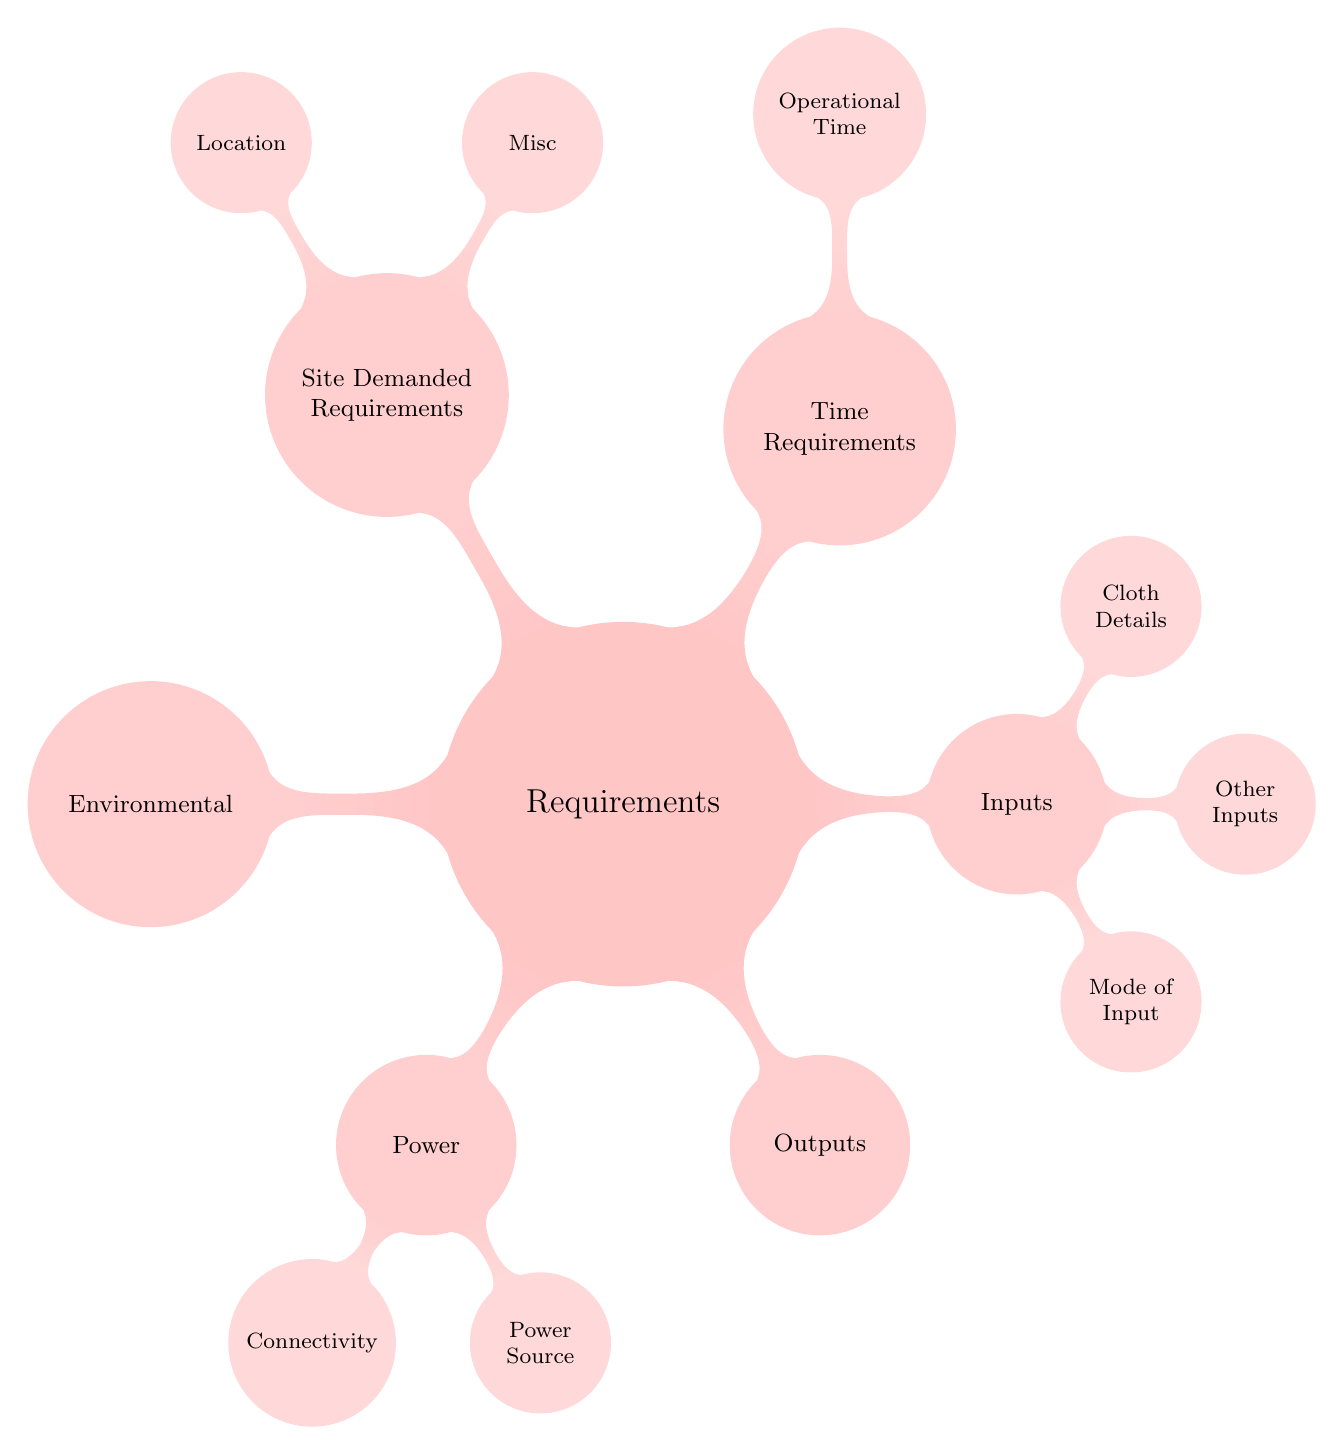
\begin{tikzpicture}
  \path[mindmap,concept color=pink!90,text=black, text width=4.5cm]
    node[concept] {Requirements}
    [clockwise from=0]
    child[concept color=pink!75] {
      node[concept] {Inputs}
      [clockwise from=60]
      child[concept color=pink!60] { node[concept] {Cloth Details} }
      child[concept color=pink!60] { node[concept] {Other Inputs} }
      child[concept color=pink!60] { node[concept] {Mode of Input} }
    }
    child[concept color=pink!75] {
      node[concept] {Outputs}
      [clockwise from=0]
    }
    child[concept color=pink!75] {
      node[concept] {Power}
      [clockwise from=-60]
      child[concept color=pink!60] { node[concept] {Power Source} }
      child[concept color=pink!60, text width=2cm] { node[concept] {Connectivity} }
    }
    child[concept color=pink!75, text width=3cm, level distance=6cm] {
      node[concept] {Environmental}
      [clockwise from=180]
    }
    child[concept color=pink!75, text width=2.9cm, level distance=6cm] {
      node[concept] {Site Demanded Requirements}
      [clockwise from=120]
      child[concept color=pink!60, level distance=3.7cm] { node[concept] {Location} }
      child[concept color=pink!60, level distance=3.7cm] { node[concept] {Misc} }
    }
    child[concept color=pink!75, text width=2.75cm, level distance=5.5cm] {
      node[concept] {Time \\Requirements}
      [clockwise from=90]
      child[concept color=pink!60, text width=2cm, level distance=4cm] {
      node[concept] {Operational Time} }
    };
\end{tikzpicture}
    \caption{Mind Map}
    \label{fig:mindmap}
\end{figure}
% \section{Glossary}
\newpage
\section{Project Management Details}
\subsection{Gantt Chart}
\begin{center}
    \begin{figure}[H]
        \centering
        \includegraphics[width=1.05\linewidth]{Images/Gantt Chart (1)_1.jpg}
        \caption{GANTT Chart}
        \label{fig:ganttchart}
    \end{figure}
\end{center}

\subsection{Network Chart}
\begin{center}
    \begin{figure}[H]
        \centering
        \includegraphics[width=1.05\linewidth]{Images/NetworkChart_1.jpg}
        \caption{Network Chart}
        \label{fig:networkchart}
    \end{figure}
\end{center}

\subsection{RBS}
\begin{center}
    \begin{figure}[H]
        \centering
        \includegraphics[width=1\linewidth]{Images/RBS_1.jpg}
        \caption{Resource Breakdown Structure}
        \label{fig:rbs}
    \end{figure}
\end{center}

\subsection{WBS}
\begin{center}
    \begin{figure}[H]
        \centering
        \includegraphics[width=1.1\linewidth]{Images/WBS_1.jpg}
        \caption{Work Breakdown Structure}
        \label{fig:wbs}
    \end{figure}
\end{center}
\section{Abstract}
The goal of this project is to create an effective cloth cleaning equipment specifically for treating white unbleached cotton cloth after production. The cloth needs a particular cleaning procedure because of its unique size, thread count, and ingrained oil-based stains imbued during manufacturing. The machine, intended for semi-industrial settings, needs to be quick to use, use less resources, and adhere to environmental rules. Time efficiency being of utmost importance, each batch must complete a full washing and drying cycle in less than 45 minutes.

\section{Motivation}
The motivation behind this cloth cleaning machine design project is rooted in addressing a practical need within the textile industry. Manufacturing uncolored cotton cloth presents unique challenges, with oil-based stains acquired during the manufacturing process requiring specialized cleaning. The pursuit of an efficient and tailored solution stems from a commitment to innovation. \\ \\By developing a machine specifically designed for post-manufacturing treatment, we aim to enhance the overall quality and cleanliness of the cloth. The project's focus on utilizing minimal resources aligns with our commitment to environmental responsibility, ensuring compliance with regulatory standards. The project's scope extends beyond technical efficiency. We envision a cloth cleaning machine that caters to the needs of semi-industrial sites. Furthermore, the motivation is fueled by the aspiration to contribute to time efficiency. With a targeted washing and drying cycle of under 45 minutes per batch, we seek to streamline operations and enhance productivity in textile processing.
\section{Requirements}
\subsection{Problem Statement}
\begin{center}
    \textbf{``Design and Manufacture a machine to clean manufacturing stains off an unbleached cotton cloth ''}
\end{center}

\subsection{Input Requirements}
\subsubsection{Cloth Details}
\begin{itemize}
    \item[$\scriptstyle\circ$] The cloth being cleaned is just-manufactured, uncolored cotton cloth, for general usage. The thickness is 1-ply, with a thread count of 400, and of denier 60 opaqueness.
    \item[$\scriptstyle\circ$] The dimensions of the cloth to be cleaned are a maximum of 10m length and 2m width or a continuous roll of 2m width.
    \item[$\scriptstyle\circ$] Cloth, if uncut, needs to be cut to 10m x 2m size.
    \item[$\scriptstyle\circ$] The cloth has mostly oil-based stains, to begin with, naturally imbued during the manufacturing process.
\end{itemize}
\subsubsection{Other inputs}
\begin{itemize}
    \item[$\scriptstyle\circ$] The machine works with pressured water available at an ambient temperature from a 35m overhead tank of capacity 50l on-site. 
    \item[$\scriptstyle\circ$] The machine works with water of $80mg/l$ $CaCO_3$ equivalent hardness.
    \item[$\scriptstyle\circ$] Expendable materials like detergents, soaps, etc are to be treated as a running cost, and paid for by the client after installation.
\end{itemize}
\subsubsection{Mode of Input}
\begin{itemize}
    \item[$\scriptstyle\circ$] The machine cleans in batches of 11 Kg dry weight per batch.
    \item[$\scriptstyle\circ$] Only a single program for general washing is required.
    \item[$\scriptstyle\circ$]The machine is required to have the capability to sequentially process multiple batches prepared beforehand by the client. 
\end{itemize}

\subsection{Output Requirements}
\begin{itemize}
    \item[$\scriptstyle\circ$] The machine is required to both wash and dry the cloth. 
    \item [$\scriptstyle\circ$] The 10m x 2m output cloth needs to be rolled.
    \item [$\scriptstyle\circ$] The output should be bone-dry.
\end{itemize}
\subsection{Power Requirements}
\begin{itemize}
    \item[$\scriptstyle\circ$] The machine must be compatible with 220V AC 1-$\Phi$ (desirable) and 440V AC 3-$\Phi$ power drawing a maximum current of 15A.
    \item[$\scriptstyle\circ$] The machine must be able to be connected to plug points up to 20m away. 
\end{itemize}
%\subsection{Logistical Requirements}
\subsection{Environmental Requirements}
\begin{itemize}
    \item[$\scriptstyle\circ$] The machine must use as low an amount of resources(water, electricity) as possible, and comply with CPCB Regulations. 
\end{itemize}
\subsection{Site-Demanded Requirements}
\begin{itemize}
    \item[$\scriptstyle\circ$] The machine is designed to be used at semi-industrial sites. 
    \item[$\scriptstyle\circ$] The machine must produce a maximum noise intensity of 70dB. 
    \item[$\scriptstyle\circ$] The machine is desired to be disassembleable and re-installable on request. 
\end{itemize}
\subsection{Structural Requirements}
\begin{itemize}
    \item[$\scriptstyle\circ$] The machine must be of maximum dimensions 25m x 40m x 60m, designed to be installed in an industrial-size enclosure, or an open courtyard. 
\end{itemize}
\subsection{Time Requirements}
\subsubsection{Operational Time}
    \begin{itemize}
        \item[$\scriptstyle\circ$] The maximum time to wash and dry a batch must be under 45 minutes. 
    \end{itemize}
%\subsubsection{Time to Market Requirements}
%\subsubsection{Life Time Requirements}
%\subsubsection{End of Life Requirements}
% \subsection{Miscellaneous Requirements}

\newpage
\appendix
\section{Appendix}
\subsection{Document ID}
\begin{itemize}
    \item Document Type - Private Release
    \item Document Authorised by : Samarth Singla
    \item Publication Date : 13 January 2024
    \item Version Number 1.0
\end{itemize}
\subsection{Document Statistics}
\begin{itemize}
    \item Number of words = 716
    \item Number of Sentences = 77
    \item Number of Characters = 4576
\end{itemize}
\subsection{Readability Indices}
\begin{table}[H]

\begin{center}
\begin{tabular}{|l|l|l|}
\hline
\textbf{Index}              & \textbf{Value} & \textbf{Range} \\ \hline
Automated Readability Index & 12.7            & 5-22           \\ \hline
Gunning-Fog Index           & 10.23           & 0-20           \\ \hline
Flesch Reading Ease         & 85.7           & 0-100          \\ \hline
Coleman Liau Index          & 19.39          & 0-17+          \\ \hline
\end{tabular}
\end{center}
\end{table}

\end{document}